\documentclass[table]{beamer}
%\documentclass[14pt,handout]{beamer}
\usetheme{Darmstadt}
\usepackage{graphicx}
\usepackage{hyperref}
\usepackage[german]{babel}
\usepackage[T1]{fontenc}
\usepackage[utf8]{inputenc}
\setbeamertemplate{footline}[frame number]
%\usepackage{enumitem}

\usepackage{pdfcomment}
\newcommand{\ben}[1]{\pdfcomment[author=Ben]{#1}}
\newcommand{\cc}[1]{\includegraphics[height=4mm]{img/#1.png}}
\usepackage{ifthen}
\newcommand{\license}[2][]{\\#2\ifthenelse{\equal{#1}{}}{}{\\\scriptsize\url{#1}}}
\newcommand{\Cc}[1]{\begin{center}
    \includegraphics[height=20mm]{img/200px-Cc-#1.png}
\end{center}}
\usepackage{textcomp}

\usepackage{multirow}
\usepackage{xcolor}


\title{Freie Lizenzen bei Lehr- und Lernmaterialien}
\author{Chaos Computer Club Dresden\\Marius Melzer, Paul Schwanse, Stephan Thamm\\13.03.2013}
\date{Diese Folien gibt es auch öffentlich unter: http://c3d2.de/schule.html}

\begin{document}
\maketitle

\frame{\tableofcontents[hideallsubsections]}

\section{Einleitung}
\subsection{}

\begin{frame}
    \frametitle{Wissen}
    \begin{itemize}
      \item<2-> Einfache Nutzung
      \begin{itemize}
        \item<3-> Verfügbarkeit ohne Zugangsbeschränkungen
        \item<4-> Unabhängig von Zeit und Raum
        \item<5-> Weiterverteilung möglich
      \end{itemize}
      \item<6-> Kollaboratives Erstellen
      \begin{itemize}
        \item<7-> Ermöglicht durch neue Medien
        \item<8-> In gemeinschaftlichem Entwicklungsprozess
        \item<9-> Profitieren von den Änderungen anderer
      \end{itemize}
    \end{itemize}
\end{frame}
 
\begin{frame}
    \frametitle{Wer sind wir?}
    \begin{itemize}
        \item<2-> Chaos Computer Club Dresden (\url{http://c3d2.de})
            \note{}
        \item<3-> Datenspuren (\url{http://datenspuren.de})
        \item<4-> Podcasts (\url{http://pentamedia.de})
        \item<5-> Chaos macht Schule
            \begin{itemize}
                \item<2-> \url{http://ccc.de/schule}
                \item<2-> \url{http://c3d2.de/schule.html}
            \end{itemize}
            \note{alle Folien auf einmal aufblättern? Ben's vorschlag}
        \item<6-> Keine Rechtsanwälte
    \end{itemize}
\end{frame}

\begin{frame}
    \frametitle{Chaos macht Schule}
    \begin{itemize}
        \item<2->Ziele:
            \begin{itemize}
                \item<3-> Kinder auf das Internet vorbereiten \ldots
                \item<4-> \ldots nicht das Internet auf Kinder
                    \note{Scheren-Vergleich}
                \item<5-> Informationelle Selbstbestimmung
                \item<6-> Medienkompetenz
                    \note{Medium nicht nur benutzen, sondern auch verstehen. Wir machen keinen Datenschutz-Richtlinien bei Facebook klicken Vortrag!}
                \item<7-> Kreativer Umgang mit Technik
                    \note{Eigene Dinge schaffen, weg von der Konsum-Mentalität}
            \end{itemize}
        \item<8-> Schulklassen
        \item<9-> Elternabende
        \item<10-> Lehrerfortbildung
        \item<11-> Keine Rechtsberatung
    \end{itemize}
\end{frame}

\section{Creative Commons}
\subsection{}

\begin{frame}
    \begin{center}\Large
    Creative Commons
    \end {center}
\end{frame}

\begin{frame}
    \frametitle{Creative Commons}
    \begin{itemize}
        \item<2-> Organisation hat sich zum Ziel gesetzt, Lizenzen zu erarbeiten
        \item<3-> Eine Lizenz, die ...
            \begin{itemize}
                \item<5-> das Urheberrecht ergänzt (nicht ersetzt)
                \item<6-> eindeutig ist
                \item<7-> leicht verständlich ist
                \item<8-> Nutzung von Werken regelt
            \end{itemize}
        \item<9-> Besteht aus 4 Modulen: BY, SA, ND, NC
    \end{itemize}
\end{frame}

\begin{frame}
    \frametitle{Modul 1: BY (By)}
    \begin{itemize}
        \item Namensnennung des Original Urhebers
        \item implizit ab CC 3.0
        \item Urheberverweis kann auf Wunsch zurückgezogen werden
    \end{itemize}
        \Cc{by}
\end{frame}

\begin{frame}
    \frametitle{Modul 2: SA (ShareAlike)}
    \begin{itemize}
        \item "`Weitergabe unter gleichen Bedingungen"'
        \item Werk darf frei kopiert und weitergegeben werden
        \item Werk darf in Gänze oder Auszugsweise bearbeitet und verwendet werden
        \item Die Lizenz muss unverändert beibehalten werden
    \end{itemize}
    \Cc{sa}
\end{frame}

\begin{frame}
    \frametitle{Modul 3: ND (NonDerivative)}
    \begin{itemize}
        \item "`Keine Bearbeitung"'
        \item Werk darf frei kopiert und weitergegeben werden
        \item Werk darf nicht bearbeitet werden
        \item Verwendung in einer Collage nicht möglich
    \end{itemize}
    \Cc{nd}
\end{frame}

%nd kurz erklärt
\begin{frame}
    \frametitle{Modul 4: NC (NonCommercial)}
    \begin{itemize}
        \item "`Nur nicht-kommerzielle Nutzung"'
        \item Werk darf frei kopiert und weitergegeben werden
        \item Werk darf nicht in kommerziellen Produkten vorkommen
        \item Probleme: Was ist kommerziell?
    \end{itemize}
    \Cc{nc}
\end{frame}

\begin{frame}
    \frametitle{Baukastensystem}
    \begin{itemize}
        \item<1-> Nutzungsbedingungen der Inhalte ist Nutzern klar, da diese die Lizenz erkennen
        \item<2-> Lizensierung des eigenen Werkes einfach möglich
        \item<3-> durch Kombination sind 6 Lizenzen zusammenstellbar
        \item<4-> Praxis: \url{https://creativecommons.org/choose/?lang=de}
    \end{itemize}
\end{frame}

\begin{frame}
    \frametitle{Lizensierung eigener Werke}
    \begin{itemize}
        \item<2-> Es muss vermerkt werden:
            \begin{enumerate}
                \item<3-> Original Urheber
                \item<4-> Lizenz
                \item<5-> Link zur Lizenz
            \end{enumerate}
        \item<6-> kann nicht zurückgezogen werden
        \item<7-> nicht exklusiv
        \item<8-> Maschinenlesbar durch CC REL
    \end{itemize}
\end{frame}

\begin{frame}
    \frametitle{Kompatibilität zwischen Lizenzen}
    \begin{center}
        \begin{tabular}{ c l|c cccccc }
            \multicolumn{2}{c|}{}&  \multicolumn{7}{ c }{Lizenzen neues Werk} \\
            \multicolumn{2}{c|}{Orig. Lizenz}& by & by-nc & by-nc-nd & by-nc-sa & by-nd & by-sa & pd \\
            \hline
            \multirow{7}{*}{} & pd & X & X & X & X & X & X & X \\
            & by & X & X & X & X & X & X &  \\
            & by-nc &  & X & X & X &  &  &  \\
            & by-nc-nd &  &  &  &  &  &  &  \\
            & by-nc-sa &  &  &  & X &  &  &  \\
            & by-nd &  &  &  &  &  &  &  \\
            & by-sa &  &  &  &  &  & X &  \\
        \end{tabular}
    \end{center}
\end{frame}

\begin{frame}
    \frametitle{Weitere freie Lizenzen}
    \begin{itemize}
        \item<2-> Open Database License (ODbL)
        \item<3-> Charityware
        \item<4-> Pizzaware
        \item<5-> Eigene Lizenztexte und Derivate
        \item<6-> Unbekannte Lizenzen sind Mehraufwand für Nutzer
    \end{itemize}
\end{frame}

\section{Inhalte finden}
\subsection{}

\begin{frame}
  \frametitle{Open Educational Resources}
    \begin{itemize}
        \item<2-> Materialien sind wie folgt zugänglich:
            \begin{itemize}
                \item<3-> ohne Einschränkung
                \item<4-> in einem freien Format
                \item<5-> unter einer offenen Lizenzen 
            \end{itemize}
        \item<6-> Begriff umfasst alle Arten von (Lehr-)Materialien
        \item<7-> Idee: Wissensunterschiede zwischen Industrienationen und Entwicklungsländern abbauen
        \item<8-> 2007: Cape Town Open Education Declaration
        \item<9-> Beispiel: Polen lässt Unis freie Lehrmaterialien erstellen
    \end{itemize}
\end{frame}

\begin{frame}
    \begin{center}\Large
    CC-Inhalte finden
    \end {center}
\end{frame}

\begin{frame}
    \begin{center}\Large
      http://search.creativecommons.org/
    \end {center}
\end{frame}

\begin{frame}
  \frametitle{Wikimedia Commons}
  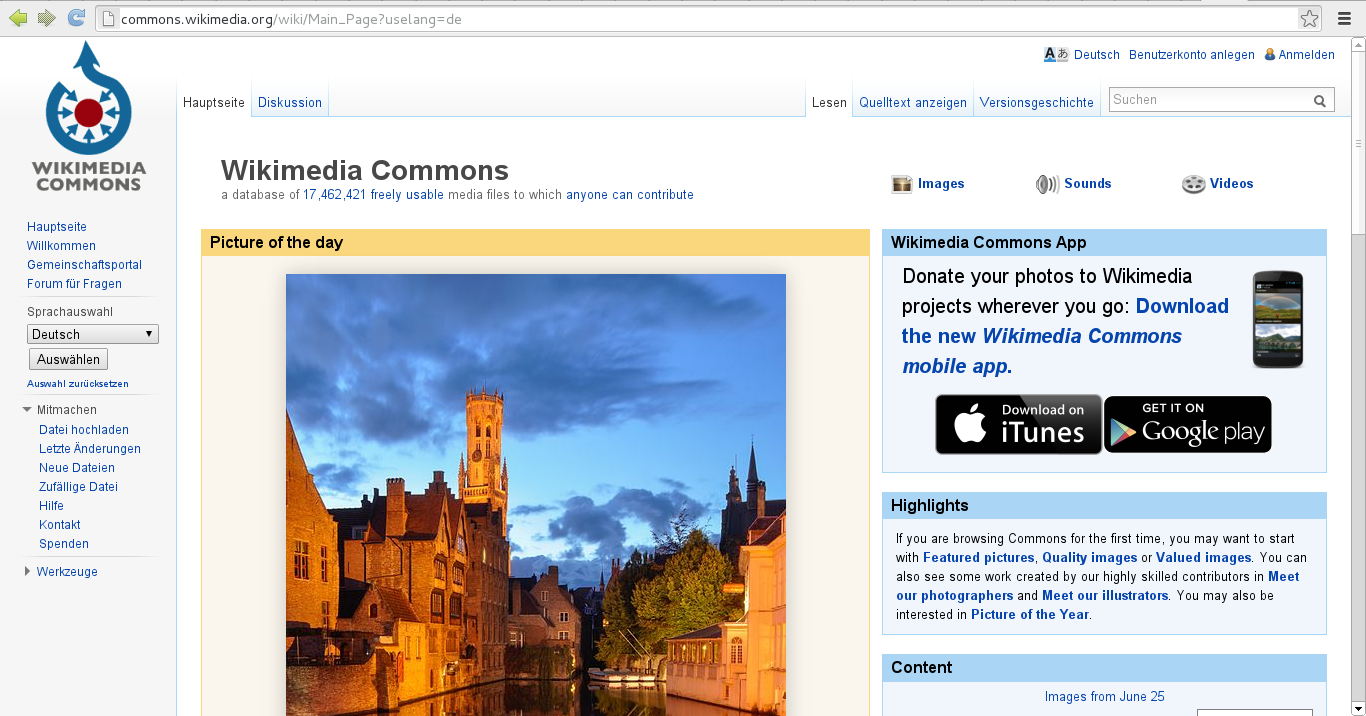
\includegraphics[width=\textwidth]{img/wikicommons.png}
\end{frame}

\begin{frame}
    \begin{center}\Large
      https://archive.org
    \end {center}
\end{frame}

\begin{frame}
    \begin{center}\Large
      http://de.wikisource.org
    \end {center}
\end{frame}

\begin{frame}
  \frametitle{Edutags}
  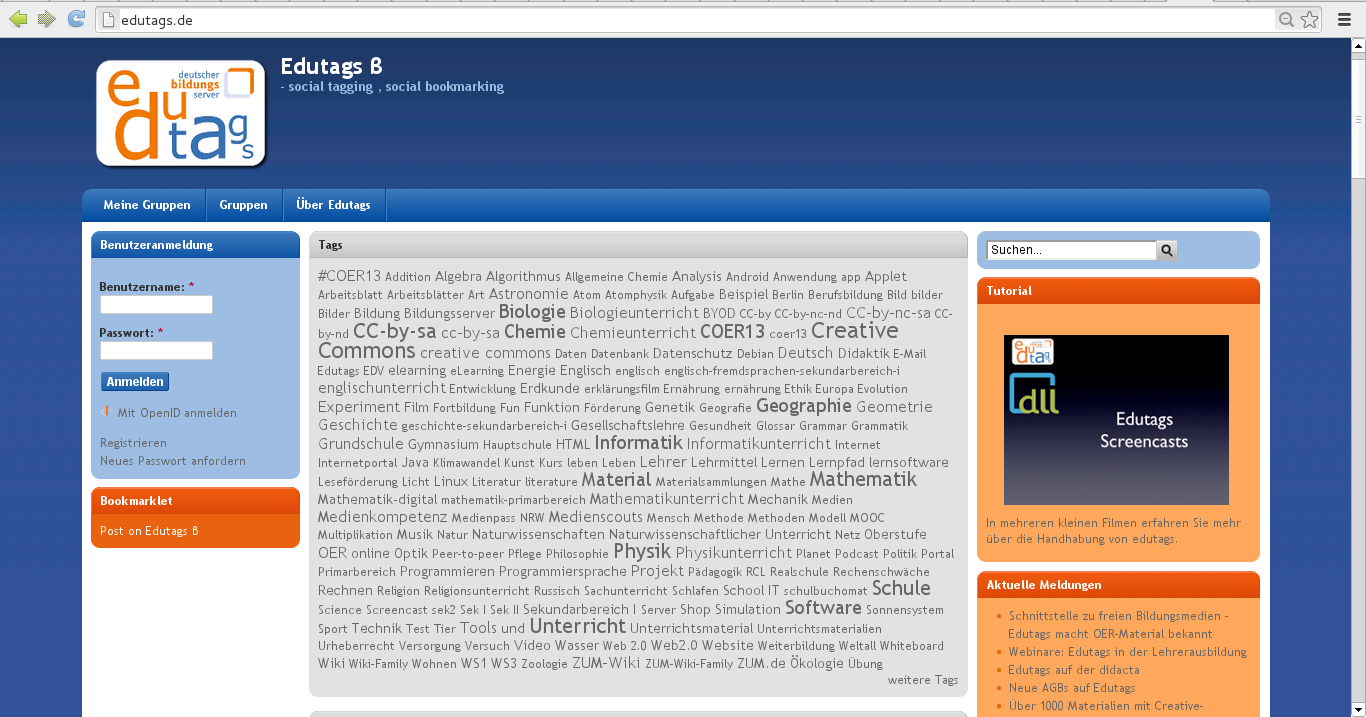
\includegraphics[width=\textwidth]{img/edutags.png}
\end{frame}

\begin{frame}
  \frametitle{Bücher}
  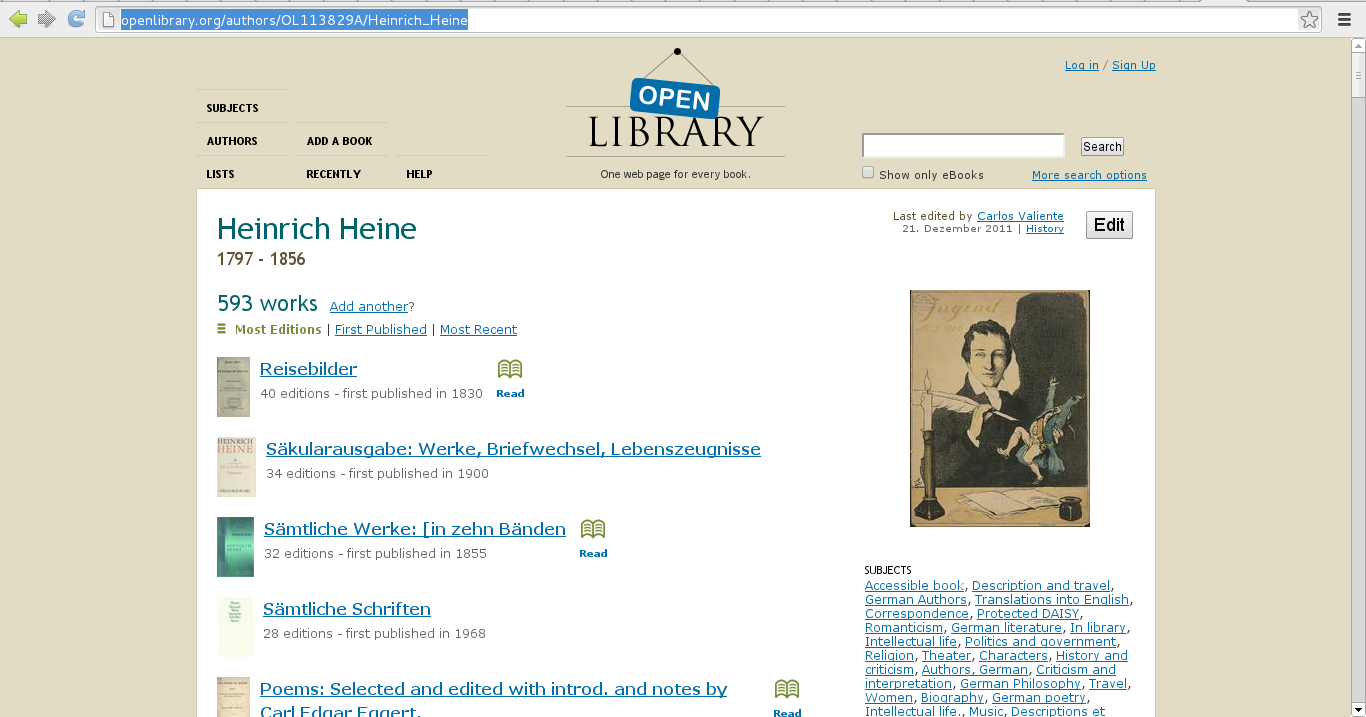
\includegraphics[width=\textwidth]{img/openlibrary.png}
\end{frame}

\begin{frame}
  \frametitle{Bücher}
  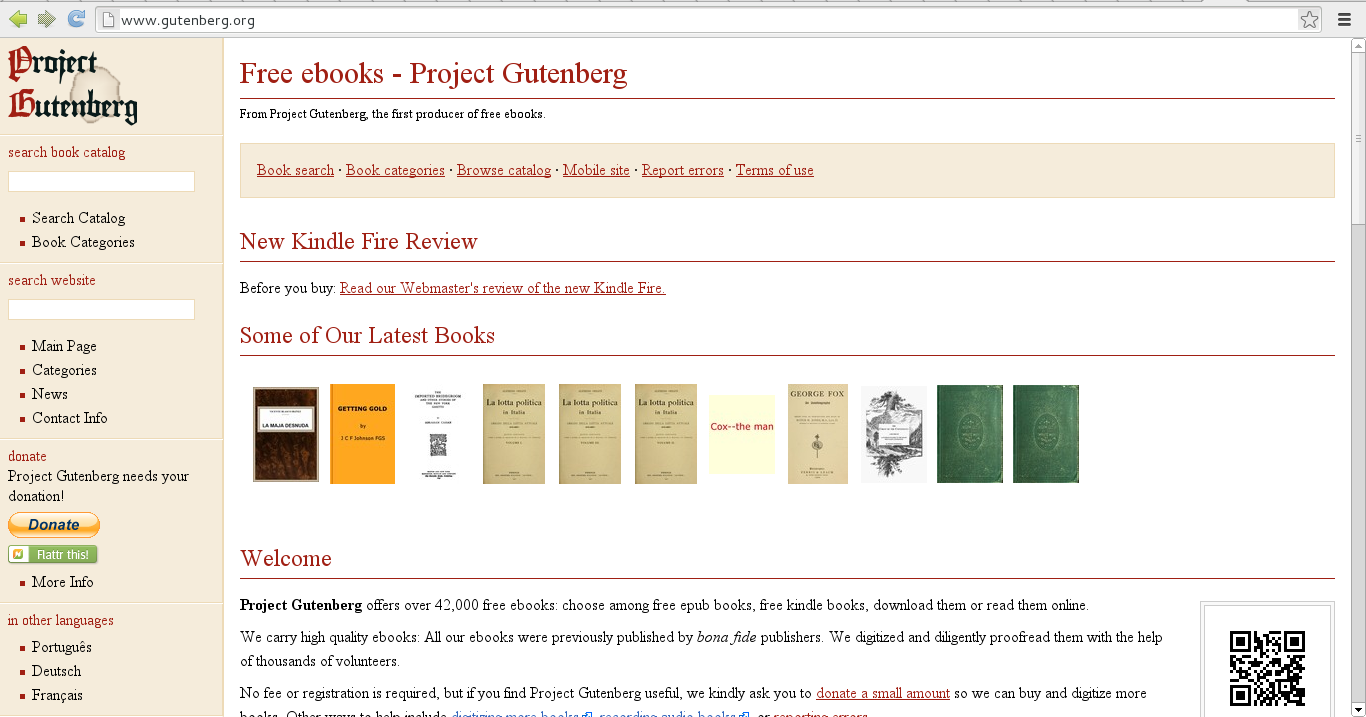
\includegraphics[width=\textwidth]{img/gutenberg.png}
\end{frame}

\begin{frame}
  \frametitle{Bücher}
  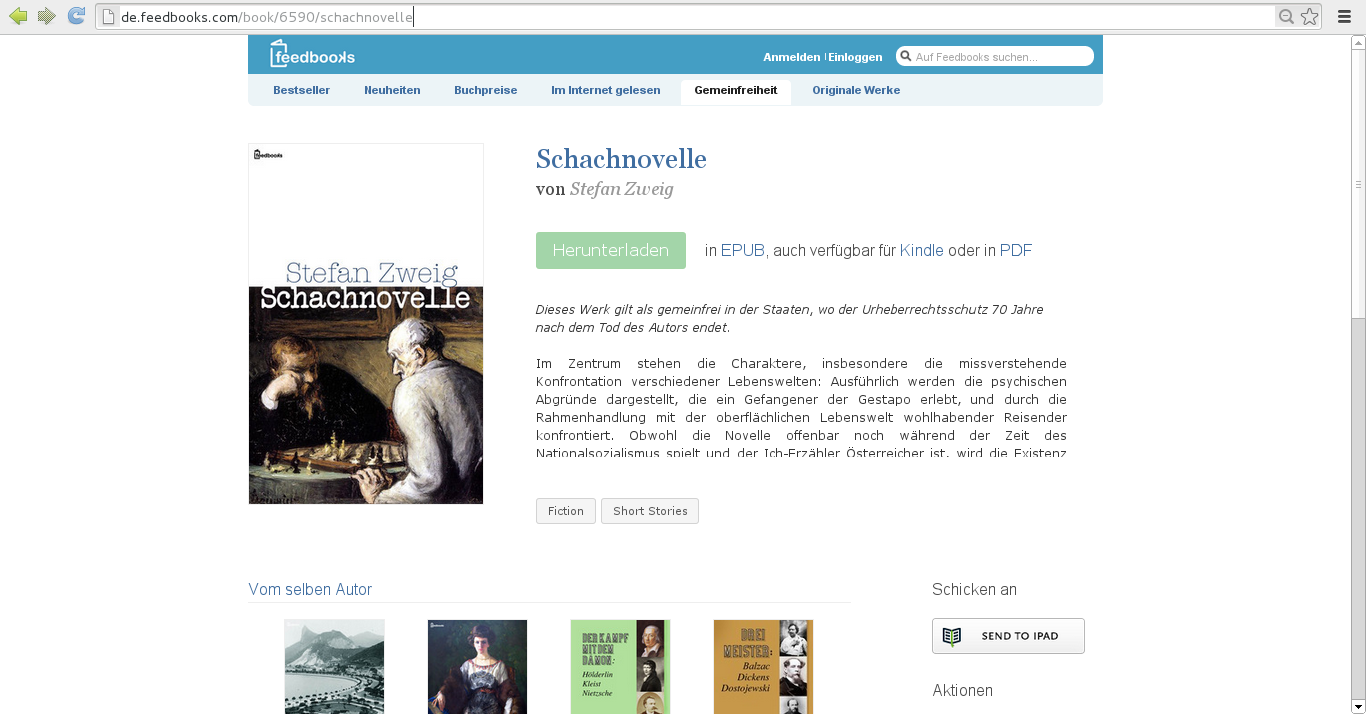
\includegraphics[width=\textwidth]{img/feedbooks.png}
\end{frame}

\begin{frame}
    \frametitle{Open Courseware}
      \begin{itemize}
        \item<2-> Berkley: http://webcast.berkeley.edu/
        \item<3-> MIT: http://ocw.mit.edu
        \item<4-> (timm: http://timms.uni-tuebingen.de/)
        \item<5-> (Coursera: https://www.coursera.org/)
    \end{itemize}
\end{frame}

\begin{frame}
    \frametitle{Weiteres}
      \begin{itemize}
        \item<1-> CC Content Directories: http://wiki.creativecommons.org/Content\_Directories
        \item<2-> Bundesarchiv: http://bundesarchiv.de
      \end{itemize}
\end{frame}

\section{Selbst Lizensieren}
\subsection{}

\begin{frame}
    \begin{center}\Large
    Selbst Lizensieren
    \end {center}
\end{frame}

\begin{frame}
    \begin{center}\Large
    http://creativecommons.org/choose/
    \end {center}
\end{frame}

\section{Fazit}
\subsection{}

\begin{frame}
    \frametitle{Fazit}
    \begin{itemize}
      \item<2-> Lizenzen zum einfachen ``Befreien'' von Inhalten
      \item<3-> Wissen baut auf Wissen auf
      \item<4-> Viele Angebot Englisch
      \item<5-> Prosument
    \end{itemize}
\end{frame}

\begin{frame}
    \frametitle{Diskussion}
    \begin{itemize}
        \item Vielen Dank für ihre Aufmerksamkeit
        \item \url{http://c3d2.de/schule.html}
        \item \url{schule@c3d2.de}
        \item Für weitere Informationen (u.a. diese Folien) besuchen Sie bitte \url{http://c3d2.de/schule.html}
    \end{itemize}
    \begin{center}
   Folien vom Chaos Computer Club Dresden\\
   {\cc{by-sa}}
   \end{center}
\end{frame}

\end{document}
